\documentclass{article}

\usepackage{amsmath,amssymb,graphicx,geometry,enumitem,caption,subcaption}
\usepackage{xepersian}

\newcounter{qnumber}
\setcounter{qnumber}{1}

\newcommand{\Q}{
\textbf{سوال \theqnumber)}
\stepcounter{qnumber}
}

\setlength{\parindent}{0mm}
\setlength{\parskip}{3mm}
\settextfont{XB Niloofar}

\begin{document}

\begin{center}
\large

به نام او

آزمون پایان ترم سیگنال ها و سیستم ها
\end{center}

\hrulefill

\large



تابع انتقال یک سیستم گسسته و LTI ، دارای نمودار صفر-قطب به صورت زیر است:

\begin{center}
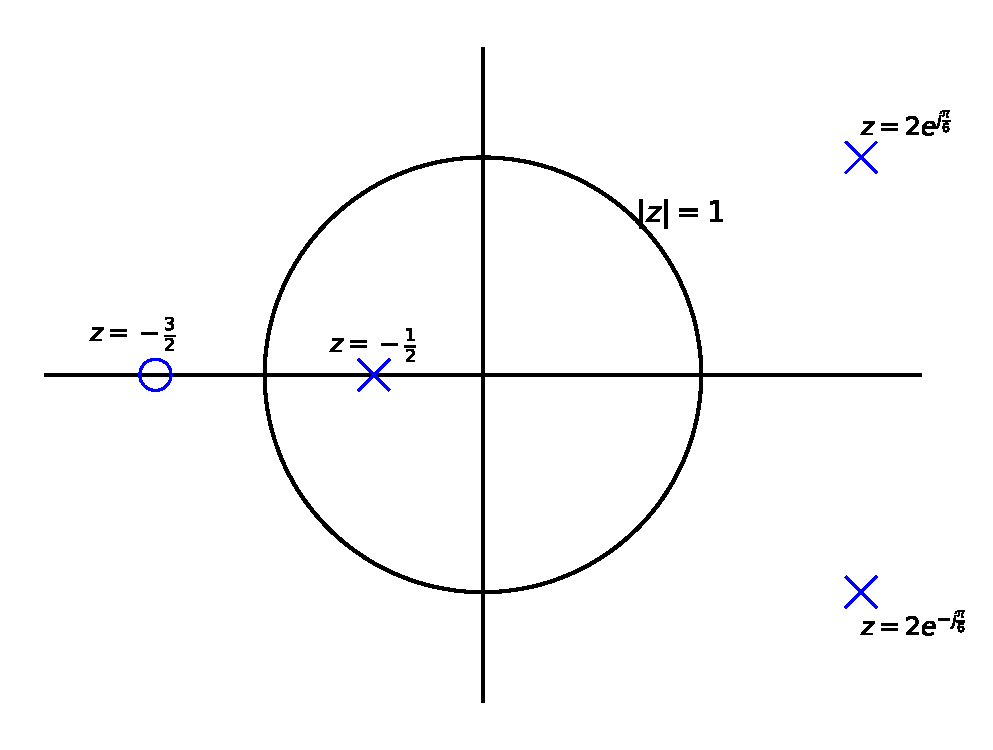
\includegraphics[width=80mm]{final_inv.eps}
\end{center}

الف) اگر سیستم علی باشد، رابطه‌ی زمانی پاسخ ضربه را بیابید.

ب) اگر سیستم پایدار و دارای وارون پایدار باشد، رابطه‌ی زمانی پاسخ ضربه‌ی سیستم معکوس را بیابید.
\end{document}